\documentclass{article}
\usepackage[utf8]{inputenc}
\usepackage[margin=1.2in]{geometry}
\usepackage{hyperref}
\usepackage{listings}
\usepackage{xcolor}
\usepackage{minted}
\usepackage{caption}
\usepackage{subcaption}


\usepackage{tikz}
\usetikzlibrary{positioning}

\usepackage{natbib}
\usepackage{graphicx}
\usepackage{amsmath}

\usepackage{listings}
\usepackage{xcolor}

\definecolor{codegreen}{rgb}{0,0.6,0}
\definecolor{codegray}{rgb}{0.5,0.5,0.5}
\definecolor{codepurple}{rgb}{0.58,0,0.82}
\definecolor{backcolour}{rgb}{0.95,0.95,0.92}

\lstdefinestyle{mystyle}{
    backgroundcolor=\color{backcolour},   
    commentstyle=\color{codegreen},
    keywordstyle=\color{magenta},
    numberstyle=\tiny\color{codegray},
    stringstyle=\color{codepurple},
    basicstyle=\ttfamily\footnotesize,
    breakatwhitespace=false,         
    breaklines=true,                 
    captionpos=b,                    
    keepspaces=true,                 
    numbers=left,                    
    numbersep=5pt,                  
    showspaces=false,                
    showstringspaces=false,
    showtabs=false,                  
    tabsize=2
}

\lstset{style=mystyle}


\title{\vspace{-2 cm}Universidade Federal de Ouro Preto \\ Inteligência Artificial \\ Prova 2}
\author{Prof. Rodrigo Silva}
\date{}


\begin{document}

\maketitle


\begin{enumerate}
    
    \item Considere o problema de encontrar um caminho no labirinto abaixo. O objetivo é ir da posição \textbf{s} até a posição \textbf{g}. O agente pode se mover horizontalmente e verticalmente. 
    
    \begin{enumerate}
        
        \item (0.5pt) No labirinto abaixo, numere os nós expandidos (visitados) por um agente que implementa o algoritmo de busca em profundidade. A ordem das ações é para cima, para a esquerda, para a direita, e para baixo. Assuma poda de ciclos e de múltiplos caminhos.
        \begin{figure}[!ht]
            \centering
            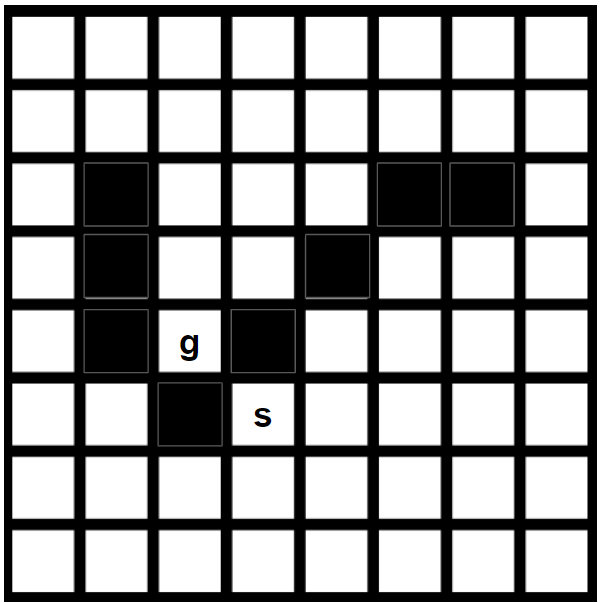
\includegraphics[width=0.37\textwidth]{lab_1.png}
        \end{figure}
        
        \item (1pt) Abaixo, (i) no labirinto da esquerda, escreva em cada nó o valor da heurística do nó, considerando a distância de Manhattan. Considere que cada quadrado tem lado 1 u.m. (ii) No labirinto da direita, numere os nós expandidos (visitados) por um agente que implementa o algoritmo $A^*$ considerando a distância de Manhattan como custo e heurística. Assuma poda de ciclos e de múltiplos caminhos.
        
     
     \begin{figure}
     \centering
     \begin{subfigure}[b]{0.45\textwidth}
         \centering
         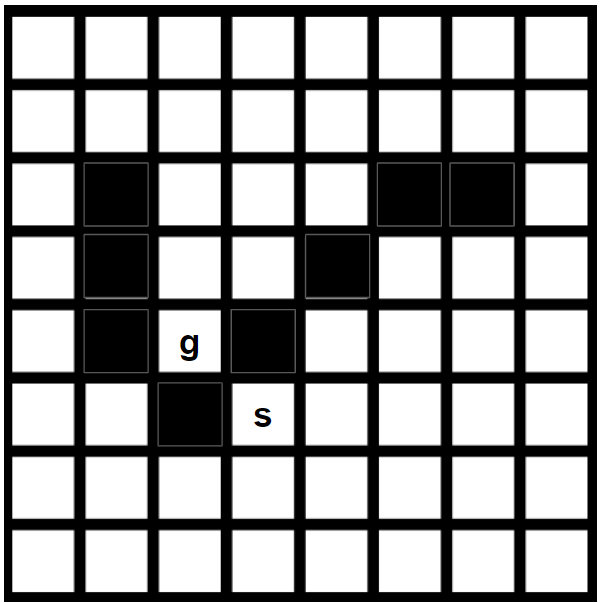
\includegraphics[width=0.8\textwidth]{lab_1.png}
         \caption{Heurística}
         \label{fig:y equals x}
     \end{subfigure}
   \hfill
     \begin{subfigure}[b]{0.45\textwidth}
         \centering
         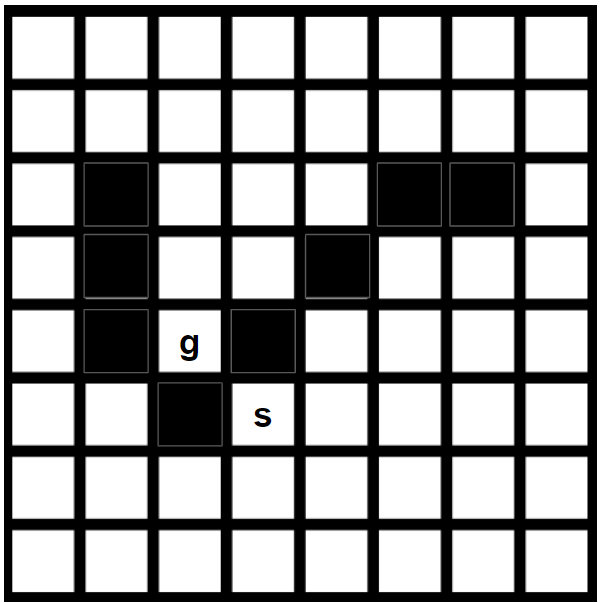
\includegraphics[width=0.8\textwidth]{lab_1.png}
         \caption{A$^*$}
         \label{fig:three sin x}
     \end{subfigure}
     \label{fig:three graphs}
     \end{figure}
        
        
    \end{enumerate}
    
    \pagebreak
    
    \item (0.5pt) Apresente o pseudocódigo de um algoritmo genérico de busca local.
    
    \begin{tikzpicture}
    \draw (0,0) -- (15,0) -- (15,9) -- (0,9) -- (0,0);
    \end{tikzpicture}
    
    \item (0.5pt) Apresente uma formulação do problema das n-rainhas e apresente a rede (grafo) de restrições considerando o problema das \textbf{3-rainhas}.
        
    \begin{tikzpicture}
    \draw (0,0) -- (15,0) -- (15,10.5) -- (0,10.5) -- (0,0);
    \end{tikzpicture}
        
    \pagebreak    

    \item Considere a seguinte base de conhecimento (KB):
    \begin{center}
      \begin{align*}
bronchitis & \leftarrow influenza.\\
bronchitis & \leftarrow smokes.\\
coughing & \leftarrow bronchitis.\\
wheezing & \leftarrow bronchitis.\\
fever & \leftarrow influenza.\\
fever & \leftarrow infection.\\
sore\_throat & \leftarrow influenza.\\
false & \leftarrow smokes \wedge nonsmoker.\\
\textbf{assumables}&:  smokes, nonsmoker, influenza, infection.
      \end{align*}
    \end{center}
    
    
    \begin{enumerate}
        \item (0.5pt) Apresente as derivações geradas por abdução para obter todas as explicações para as observações $wheezing \wedge nonsmoker$, 
        
        \begin{tikzpicture}
        \draw (0,0) -- (14,0) -- (14,9) -- (0,9) -- (0,0);
     \end{tikzpicture}
        
        \item (0.5pt) Das explicações obtidas acima, quais são explicações mínimas. Por quê?
        
        \begin{tikzpicture}
        \draw (0,0) -- (14,0) -- (14,5) -- (0,5) -- (0,0);
     \end{tikzpicture}
        
    \end{enumerate}
    \pagebreak
    
    \item Considere a base de dados abaixo:
    
    \begin{table}[!h]
        \centering
        \begin{tabular}{c|c|c}
             $x_1$ & $x_2$ & $y$\\
             \hline
              4 & 5 & 12 \\
              3 & 8 & 17 \\
              1 & 3 & 5 \\ %x1 + 2x2 - 2
        \end{tabular}
        \label{tab:my_label}
    \end{table}
    
    \begin{enumerate}
        \item (0.5pt) Escreva a expressão genérica de um modelo linear para as variáveis deste problema.
        
        \begin{tikzpicture}
        \draw (0,0) -- (14,0) -- (14,2) -- (0,2) -- (0,0);
        \end{tikzpicture}
    
        \item (0.5pt) Escreva a expressão da soma do erro quadrado médio em função do pesos do modelo para a base de dados apresentado.
        
        \begin{tikzpicture}
        \draw (0,0) -- (14,0) -- (14,2) -- (0,2) -- (0,0);
        \end{tikzpicture}
    
        \item (0.5pt) Dado o vetor de pesos $\mathbf{w} = [1,2,3]^t$. Qual a previsão do modelo para a entrada $\mathbf{x} = [1,1,1]^t$? Qual o erro absoluto total deste modelo para a base de dados apresentada.
        
        \begin{tikzpicture}
        \draw (0,0) -- (14,0) -- (14,4) -- (0,4) -- (0,0);
        \end{tikzpicture}
        
        \item (0.5pt) Considere a biblioteca Sklearn. Descreva o que cada uma das linhas abaixo faz:
        
        \begin{figure}[!ht]
        \centering
        \inputminted[linenos]{python}{linear.py}
        \label{fig:abduction}
        \end{figure}
        
        \begin{tikzpicture}
        \draw (0,0) -- (14,0) -- (14,4) -- (0,4) -- (0,0);
        \end{tikzpicture}
        
    \end{enumerate}
    
    \item Considere a seguinte base de dados:
    
    \begin{figure}[!ht]
        \centering
        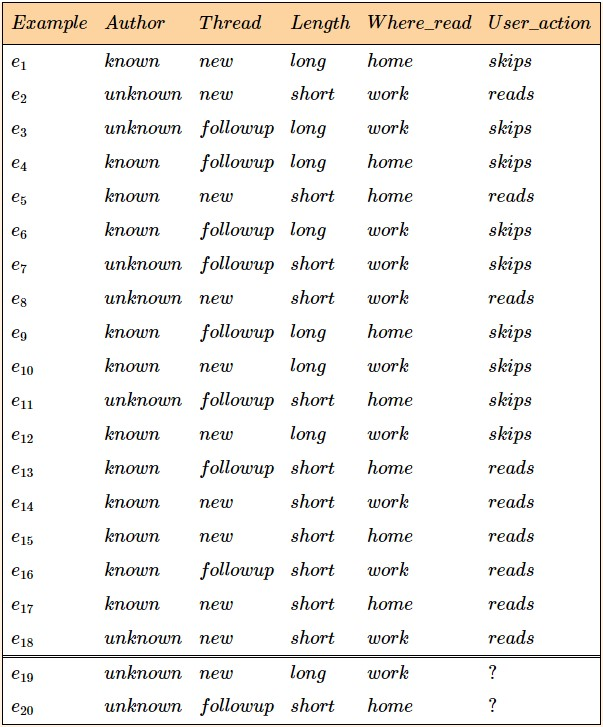
\includegraphics[width=0.55\textwidth]{abc.jpg}
    \end{figure}

    \begin{enumerate}
        \item (1 pt) Apresente uma árvore de decisão para a classificação das \textit{User-actions} e calcule o grau de impureza ($I_G$) médio do nó raiz da sua árvore. (Obs: $I_G(p) = 1 - \sum_{i=1}^{J}p_i^2$)
        
        \begin{tikzpicture}
        \draw (0,0) -- (14,0) -- (14,6.5) -- (0,6.5) -- (0,0);
        \end{tikzpicture}
        
        \item (0.25pt) De acordo com a árvore apresentada, qual a classificação dos exemplos $e_{19}$ e $e_{20}$?
        
        \begin{tikzpicture}
        \draw (0,0) -- (14,0) -- (14,1.5) -- (0,1.5) -- (0,0);
        \end{tikzpicture}
        
    \end{enumerate}
   
   \item Sobre redes neurais, responda:
   
   \begin{enumerate}
    \item (0.5pt) Como uma rede neural \textit{aprende}?
    
     \begin{tikzpicture}
        \draw (0,0) -- (14,0) -- (14,4.5) -- (0,4.5) -- (0,0);
        \end{tikzpicture}
    
    \item (0.5pt) Explique o algoritmo de descida do gradiente (\textit{Gradient Descent}).
    
    \begin{tikzpicture}
        \draw (0,0) -- (14,0) -- (14,4.5) -- (0,4.5) -- (0,0);
        \end{tikzpicture}
    
    \item (0.25pt) Para o que serve o algoritmo de \textit{back-propagation}?
    
    \begin{tikzpicture}
        \draw (0,0) -- (14,0) -- (14,4.5) -- (0,4.5) -- (0,0);
        \end{tikzpicture}
    
    \item (0.5pt) Descreva \textit{overfitting}.
    
    \begin{tikzpicture}
        \draw (0,0) -- (14,0) -- (14,4.5) -- (0,4.5) -- (0,0);
        \end{tikzpicture}
    
    \item (0.5pt) Descreva algum método de regularização e explique como ele reduz o \textit{overfitting}?
    
    \begin{tikzpicture}
        \draw (0,0) -- (14,0) -- (14,4.8) -- (0,4.8) -- (0,0);
        \end{tikzpicture}
    
    \item (0.25pt) Quais são os hiper-parâmetros de uma RNA?
    
    \begin{tikzpicture}
        \draw (0,0) -- (14,0) -- (14,4.8) -- (0,4.8) -- (0,0);
        \end{tikzpicture}
    
    \item (0.25pt) Para o que serve a técnica de \textit{drop-out}?
    
    \begin{tikzpicture}
        \draw (0,0) -- (14,0) -- (14,4.8) -- (0,4.8) -- (0,0);
        \end{tikzpicture}
    
    \item (0.25pt) O que é um \textit{minibatch}? Para o que servem os \textit{minibatches}?
    
    \begin{tikzpicture}
        \draw (0,0) -- (14,0) -- (14,4.8) -- (0,4.8) -- (0,0);
        \end{tikzpicture}
    
    \item (0.25pt) Defina taxa de aprendizagem. Qual o seu efeito no treinamento de uma rede neural?
    
    \begin{tikzpicture}
        \draw (0,0) -- (14,0) -- (14,4.8) -- (0,4.8) -- (0,0);
        \end{tikzpicture}
    
    \end{enumerate}
    
    \item (1pt) Na disciplina de inteligência artificial, quais aspectos são utilizados para avaliar a inteligência de um agente? Como eles podem ser medidos?
    
    \begin{tikzpicture}
        \draw (0,0) -- (15,0) -- (15,10) -- (0,10) -- (0,0);
        \end{tikzpicture}
    
    
\end{enumerate}




% Na leitura recomendada você deve ter lido que agentes são entidades que interagem com um ambiente. Nesta atividade você deve implementar agentes que encontram o caminho de uma posição inicial até uma posição alvo desviando de objetos. 

% Visite o repositório \url{https://github.com/rcpsilva/BCC740\_ArtificialIntelligence}, que contem o código base para esta atividade e leia atentamente o README.

% O arquivo \textit{Room.py} contém a classe \texttt{Room} que implementa um \texttt{Environment} que representa uma sala com obstáculos. Atributos importantes desta classe são:

% \begin{itemize}
%     \item \texttt{room}: É uma matriz que contém 0 nas posições livres e 0 nas posições com obstáculos.
%     \item \texttt{initial\_positon}: Posição inicial do agente na sala.
%     \item \texttt{target}: Posição em que o agente deve chegar.
% \end{itemize}

% O método de classe \texttt{initial\_percepts()} retorna:

% \begin{itemize}
%     \item \texttt{current\_position}: com a posição inicial do agente.
%     \item \texttt{target}: com a posição em que o agente deve chegar.
%     \item \texttt{neighboors} com as posições vizinhas livres. 
% \end{itemize}

% O método de classe \texttt{signal(action)} retorna:

% \begin{itemize}
%     \item \texttt{current\_position}: com a posição atual do agente.
%     \item \texttt{target}: com a posição em que o agente deve chegar.(Obs: Esta opção está aqui para modelar a possibilidade de mudança de objetivo durante a execução.)
%     \item \texttt{neighboors} com as posições vizinhas livres. 
% \end{itemize}

% Uma \texttt{action} é, da lista de vizinhos livres, a posição para onde o agente quer se mover. 

% Veja o exemplo ilustrado na figura \ref{fig:room}.

% \begin{figure}[!ht]
%     \centering
%     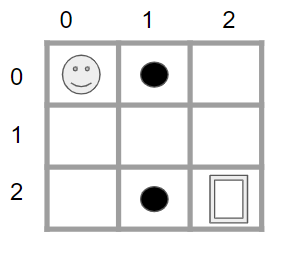
\includegraphics[width=0.4\textwidth]{room.PNG}
%     \caption{Ilustração da classe \texttt{Room}}
%     \label{fig:room}
% \end{figure}

% Para o exemplo mostrado na figura \ref{fig:room} teríamos:
%     \[
%         \texttt{room} = \begin{bmatrix}
%             0 & 1 & 0\\ 
%             0 & 0 & 0\\ 
%             0 & 1 & 0
%         \end{bmatrix}
%     \]
    
%     \[
%         \texttt{begin} = [0,0]
%     \]
    
%     \[
%         \texttt{target} = [2,2]
%     \]
    
%     \[
%         \texttt{current\_position} = [0,0]
%     \]
    
%     \[
%         \texttt{target} = [2,2]
%     \]
    
%     \[
%         \texttt{neighboors} = [[1,0],[1,1]]
%     \]

% o arquivo \textit{path\_finder\_agents.py} contém a implementação do \texttt{RandAgent}. Em cada posição, este agente escolhe um vizinho livre aleatoriamente para visitar. Ele para quando chega à posição alvo. Este agente pode ser usando como base para a implementação de outros agentes.

% Dadas estas informações, faça:

% \begin{enumerate}
%     \item Clone repositório \url{https://github.com/rcpsilva/BCC740\_ArtificialIntelligence}, leia atentamente o README e trabalhe a partir dele.
%     \item Execute o arquivo \textit{path\_finder\_simulation.py} para ver como o RandAgent se comporta.
%     \item No arquivo \textit{path\_finder\_agents.py}, implemente a classe \texttt{BFSAgent} que representa um agente que encontra a posição alvo fazendo uma busca em largura.
%     \item No arquivo \textit{path\_finder\_agents.py}, implemente a classe \texttt{DFSAgent} que representa um agente que encontra a posição alvo fazendo uma busca em profundidade.
%     \item No arquivo \textit{path\_finder\_agents.py}, implemente a classe \texttt{GreedyAgent} que representa um agente que encontra a posição alvo utilizando o algoritmo guloso.
%     \item No arquivo \textit{path\_finder\_agents.py}, implemente a classe \texttt{AStarAgent} que representa um agente que encontra a posição alvo utilizando o algoritmo A$^*$.
% \end{enumerate}

% Observações:
% \begin{itemize}
%     \item Todos os agentes implementados devem fazer poda de ciclos e poda de múltiplos caminhos.
%     \item Os agentes devem implementar a interface \texttt{Agent} definida no arquivo \textit{definitions.py}. 
%     \item Métodos auxiliares podem ser implementados para os agentes.
%     \item A classe $Room$ não deve ser modificada.
%     \item Os agentes implementados devem ser testados como indicado no arquivo \textit{path\_finder\_simulation.py}
% \end{itemize}
    

% %\bibliographystyle{plain}
% %\bibliography{references}
\end{document}

